%% Ultrainfinitism
%%
%% Render with:
%%   lualatex -shell-escape ultrainfinitism.tex \
%%     && lualatex -shell-escape ultrainfinitism.tex
%% (self-contained bibliography; no bibtex pass required)

\documentclass[]{article}
\usepackage{url}
\usepackage[hyperindex,breaklinks]{hyperref}
\IfFileExists{breakurl.sty}{\usepackage{breakurl}}{}
\usepackage{listings}
\lstset{basicstyle=\ttfamily\footnotesize,breaklines=true,frame=single,
        xleftmargin=1em,xrightmargin=0.5em}
\usepackage{float}
\restylefloat{table}
\usepackage{longtable}
\usepackage{booktabs}
\usepackage{graphicx}
\usepackage[font=small,labelfont=bf]{caption}
\usepackage[skip=0pt]{subcaption}
\usepackage{amsfonts}
\usepackage{amsmath}
\usepackage{amssymb}
\usepackage{amsthm}
\usepackage{mathtools}
\usepackage{unicode-math}
\IfFileExists{newunicodechar.sty}{
  \usepackage{newunicodechar}
  \newunicodechar{∘}{\ensuremath{\circ}}
}{}
\IfFontExistsTF{Stix Two Math}{\setmathfont{Stix Two Math}}{\setmathfont{STIX Math}}

% Compatibility fallback for older TeX bundles.
\makeatletter
\providecommand{\headerps@out}{}
\makeatother

\usepackage{tikz}
\usetikzlibrary{arrows.meta,positioning,calc,decorations.pathreplacing,fit,backgrounds}

\newtheorem{theorem}{Theorem}
\newtheorem{lemma}[theorem]{Lemma}
\newtheorem{proposition}[theorem]{Proposition}
\newtheorem{corollary}[theorem]{Corollary}
\theoremstyle{definition}
\newtheorem{definition}[theorem]{Definition}
\newtheorem{principle}[theorem]{Principle}
\theoremstyle{remark}
\newtheorem{remark}[theorem]{Remark}

\newcommand{\code}[1]{\texttt{#1}}
\newcommand{\lpath}[1]{{\ttfamily\nolinkurl{#1}}}
\newcommand{\ty}[1]{\ensuremath{\mathtt{#1}}}
\newcommand{\Uf}{\mathcal{U}}
\newcommand{\limstar}{\ensuremath{M^{\!*}}}
\newcommand{\R}{\mathbb{R}}
\newcommand{\N}{\mathbb{N}}
\DeclareMathOperator{\uprod}{\textstyle\prod}

\emergencystretch=3em

\title{Ultrainfinitism:\\
       the finite as a principal-ultrafilter shadow of the One\\[4pt]
       {\large Ultraproducts, \L o\'s transfer, and imprecise construction\\
        for conjecture, credence, and concept formation}}
\author{Mettapedia Working Notes}
\date{\today}

\begin{document}
\maketitle

\begin{abstract}
\emph{Ultrafinitism} holds that only sufficiently small finite objects are real.
\emph{Ultrainfinitism} is its inverse: only the infinite is truly real, and the
finite is a \emph{simulation}---a coordinate-shadow that a \emph{principal
ultrafilter} projects out of the One. (This anti-finitary sense is distinct from,
and nearly opposite to, an older use of the word for a programme \emph{beyond} the
transfinite; we develop the former, which has lacked a worked mathematical account.)
This essay steelmans that thesis and gives it teeth. The phenomenological motivation is direct: nothing finite is ever
\emph{given} in experience; every act of looking deeper finds more, granularity
never bottoms out, and even the discrete quanta of physics resolve, on inspection,
into excitations of continuous fields. The mathematical home is equally direct:
the ultraproduct $\bigl(\uprod_i M_i\bigr)/\Uf$ and {\L}o\'s's theorem. A
\emph{principal} ultrafilter selects a single coordinate---a finitary shadow; a
\emph{free} ultrafilter (the canonical \code{hyperfilter}) builds a genuinely
infinite object---the One; and {\L}o\'s's theorem is the law that transfers truth
between them. We show that three constructions already \emph{proved}, sorry-free,
in the Mettapedia Lean~4 development are exactly the load-bearing instances of this
picture: (i) {\L}o\'s's theorem itself, native to the repository, gives a semantics
for \emph{conjecturing in the limit}; (ii) the credal-width theorems make the
\emph{precise $=$ principal, imprecise $=$ free} dial mathematically exact; and
(iii) the de~Finetti machinery realizes the \emph{infinite-primary} construction
order in which finite-prefix laws are mere projections of one infinite measure.
We separate scrupulously what is proved from what is envisioned, and we draw out
the philosophical and practical ramifications---for automated conjecture, for
imprecise Bayesianism, and for the discrete/continuous boundary in physics and
machine learning.
\end{abstract}

\section{Prologue: nothing finite is ever given}
\label{sec:prologue}

Begin not with axioms but with attention. Try to be shown something finite---a
single, complete, bounded thing, given all at once with nothing left over. You
will not be shown it. Whatever you fix upon, you can look closer: the edge of the
table dissolves into fibre, the fibre into cellulose, the molecule into a cloud
of amplitude. At no stage does a final grain appear and announce itself as the
last. The phenomenology of perception is a phenomenology of \emph{regress}, not of
arrival.

Physics, our most disciplined looking, tells the same story when pressed. The
quantum looks like the triumph of the discrete---a smallest packet, a countable
click. But the quantum is not a pebble; it is an \emph{excitation of a field},
and the field is a continuous assignment of amplitude over all of space and time.
The particle is what a bounded, situated observer \emph{distinguishes} within an
unbounded continuum; it is a reading, not a brick. The world-crystal and
observer-relative reconstructions of quantum structure make this precise from the
physics side: local, conserved, particle-like behaviour \emph{emerges} from a
continuum substrate under the regularities an observer can resolve, rather than
the continuum being assembled from particles \cite{GoertzelWorldCrystal,
GoertzelObserverRelative}.

\begin{figure}[H]
\centering
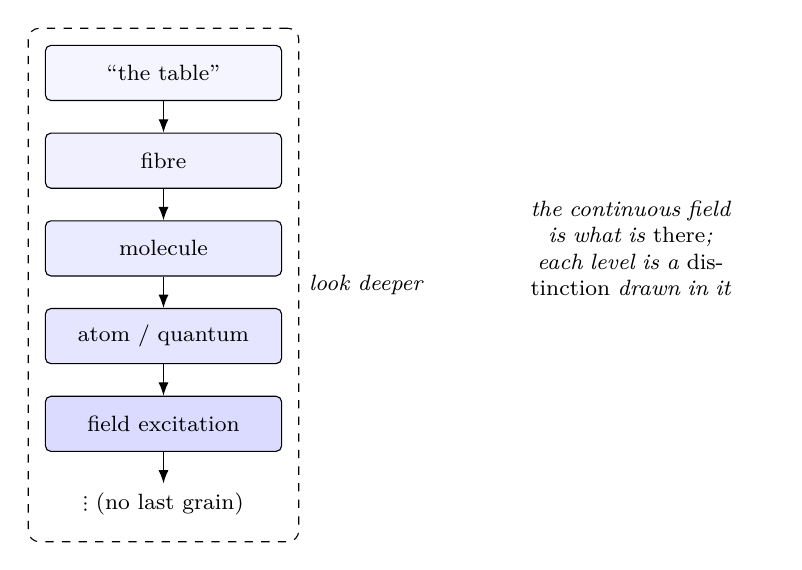
\begin{tikzpicture}[
  >=Latex, every node/.style={font=\footnotesize},
  lvl/.style={draw, rounded corners=2pt, minimum width=30mm, minimum height=7mm,
              align=center}
]
  \node[lvl, fill=blue!4] (a) {``the table''};
  \node[lvl, fill=blue!6, below=4mm of a] (b) {fibre};
  \node[lvl, fill=blue!8, below=4mm of b] (c) {molecule};
  \node[lvl, fill=blue!10, below=4mm of c] (d) {atom / quantum};
  \node[lvl, fill=blue!14, below=4mm of d] (e) {field excitation};
  \node[font=\footnotesize, below=4mm of e] (f) {$\vdots$ (no last grain)};
  \draw[->] (a)--(b); \draw[->] (b)--(c); \draw[->] (c)--(d);
  \draw[->] (d)--(e); \draw[->] (e)--(f);
  \node[draw, dashed, rounded corners, fit=(a)(f), inner sep=6pt,
        label={[font=\footnotesize\itshape]right:look deeper}] {};
  % the continuum on the right
  \node[align=center, right=26mm of c, font=\footnotesize\itshape, text width=34mm]
    {the continuous field is what is \emph{there};\\ each level is a
     \emph{distinction} drawn in it};
\end{tikzpicture}
\caption{The phenomenological regress (D5). Each finite ``object'' is a distinction
drawn within a continuum that itself never appears as a finite datum. The arrows
never terminate in a last grain.}
\label{fig:regress}
\end{figure}

The moral is not scepticism about the finite; finite descriptions are
indispensable. The moral is about \emph{priority}. The finite is something we
\emph{do}---an act of distinction performed by a situated observer---whereas the
infinite continuum is what the doing is done \emph{to}. Ultrainfinitism takes this
order of priority seriously and asks what mathematics looks like when the infinite
is the ground and the finite is the derived, simulated thing.

\section{The thesis: the Law of Oneish}
\label{sec:thesis}

\begin{principle}[Ultrainfinitism]
\label{prin:ui}
Only the infinite is truly real. Every finite object is a \emph{simulation}: a
projection of the One onto a single coordinate, effected by a \emph{principal
ultrafilter}. Distinctions---and hence finitudes---are observer-relative carvings
of an indivisible infinite whole. Call this last clause the \emph{Law of Oneish}:
beneath the carvings there is one thing, and the carvings are how a perspective
makes a finite world to live in.
\end{principle}

The thesis can be stated as a syllogism. \emph{(1)} True separation does not
obtain in the world---no boundary is absolute, every cut leaks. \emph{(2)} The
world is infinite. \emph{Therefore (3)} no truly finite, fully separated entity
exists; finitude is a working abstraction, not a fundamental fact. The number $1$,
on this reading, has its \emph{formal} home as a \emph{terminal object}: an entity
with no internal parts of its own, individuated only by the unique map into it from
every object (Section~\ref{sec:adjoint}); the looser gloss ``$1$ as the equivalence
class of all objectifiable systems counted as one'' is the intuition, not the
technical core. In a phenomenological register the same point reads as analytic
idealism: finitary distinctions are contortions in an undivided field of awareness,
useful folds rather than separate things.

The step from phenomenology to ontology should not be rushed; that ``nothing finite
is given'' supports anti-atomism and observer-relativity more directly than full
monism. We therefore separate two bridge principles and grade them honestly.

\begin{principle}[No-Atom, from No-Separation]
\label{prin:bridge1}
If no boundary is absolute---if every individual leaks into a context it cannot be
cleanly separated from---then there is no \emph{atom}: no minimal, fully separated
individual. This is the well-supported, anti-atomist core; phenomenology presses it
directly. It yields \emph{atomlessness} (Section~\ref{sec:gunk}), not yet monism.
\end{principle}

\begin{principle}[Priority of the Whole]
\label{prin:bridge2}
The infinite whole is prior to its finite carvings: a carving presupposes the
manifold it carves, but the manifold does not presuppose any particular carving.
This is the substantive metaphysical commitment that turns anti-atomism into
ultrainfinitism proper. We flag it as a commitment, argued for but not forced by the
phenomenology alone.
\end{principle}

\begin{remark}[a note on the term]
\label{rem:term}
``Ultrainfinitism'' has been used in two nearly opposite senses. In a 2012
MathOverflow discussion the word names a \emph{trans-transfinite} programme---a step
\emph{beyond} the cumulative hierarchy $V$, postulating hyper-cardinal or
``ultimate-class'' size notions larger than any ordinary cardinal, with the
hyperuniverse programme, universal-set theories, and $V\!\to\!V$ wholeness axioms as
neighbours \cite{MannucciMO2012}. The sense developed here is the
\emph{anti-finitary} one of the contemporary \texttt{\#UltraInfinitism} stance: not
bigger infinities beyond $V$, but the claim that \emph{the finite does not
fundamentally exist}. Across the available informal sources this second sense
has circulated as a metaphysical slogan rather than a worked mathematical program,
against the mature philosophical backdrop of debates over actual versus potential
infinity \cite{SEPInfinity}. Supplying such a program---an ultraproduct semantics
with proven anchors and a type-theoretic home---is the contribution of this essay.
\end{remark}

This inverts the usual constructional order. Carnap's \emph{Aufbau} and its modern
descendant, Chalmers's scrutability programme, build the world \emph{up} from a
compact base by a priori entailment \cite{Carnap1928, Chalmers2012}; Russell's
``supreme maxim'' urges us to replace inferred entities with \emph{constructions}
out of what is given \cite{Russell1914}. Ultrainfinitism keeps the constructional
spirit but reverses the arrow: the base is not a stock of finite givens from which
the infinite is approached, but the infinite One from which the finite is
\emph{projected down}. The technical engine of that projection is the ultrafilter,
to which we now turn.

\section{The mathematical home: ultraproducts, ultrafilters, \L o\'s}
\label{sec:math}

Let $(M_i)_{i\in I}$ be a family of structures and $\Uf$ an ultrafilter on the
index set $I$. The \emph{ultraproduct} $\bigl(\uprod_i M_i\bigr)/\Uf$ is the
product quotiented by the relation ``agree on a $\Uf$-large set of
coordinates.'' Two extremes govern its character.

\begin{itemize}
\item A \emph{principal} ultrafilter $\Uf=\{\,S : i_0\in S\,\}$, generated by a
single index $i_0$, collapses the ultraproduct to the single factor
$M_{i_0}$. It \emph{simulates the finitary}: the One is read off at one
coordinate, and what you get back is exactly one finite shadow.
\item A \emph{free} (non-principal) ultrafilter---canonically the
\code{hyperfilter}, extending the cofinite filter on an infinite index set---ignores
every finite set of coordinates and builds a genuinely new, infinite object: the
\emph{One}. Robinson's hyperreals are the paradigm: $\R^{\!*}=\bigl(\uprod_{n}
\R\bigr)/\,\code{hyperfilter}$, an ordered field with genuine infinitesimals and
infinities \cite{Robinson1966, Goldblatt1998, Keisler}. In our Lean dependency this
identification is literal: the type of hyperreals is defined as
\code{Germ (hyperfilter $\N$) $\R$}.
\end{itemize}

\begin{remark}[the One has genuinely new inhabitants]
\label{rem:hyperreal}
The free pole is not a re-labelling of the finite. In $\R^{\!*}$ the sequence
$\omega:=[\langle 1,2,3,\dots\rangle]$ exceeds every standard real (for each
$n_0\in\N$ the set $\{n : n>n_0\}$ is cofinite, hence in the \code{hyperfilter}, so
$\omega>n_0$), and $\varepsilon:=[\langle 1,\tfrac12,\tfrac13,\dots\rangle]$ is a
positive infinitesimal with $\omega\varepsilon=[\langle 1,1,1,\dots\rangle]=1$.
Yet every first-order truth about $\R$---the ordered-field axioms, every algebraic
identity---transfers to $\R^{\!*}$ by {\L}o\'s (Theorem~\ref{thm:los}). This is the
Law of Oneish in miniature: the One contains objects no coordinate does, while
preserving exactly the first-order shadow each coordinate sees.
\end{remark}

\begin{figure}[H]
\centering
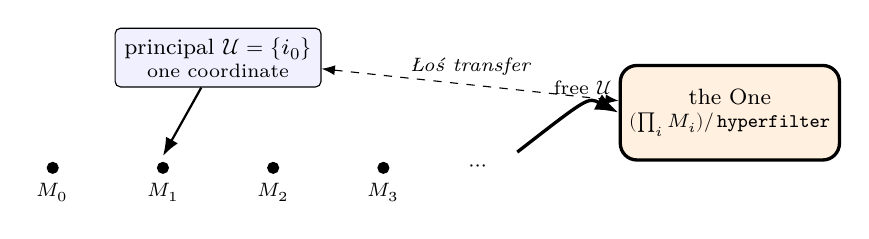
\begin{tikzpicture}[
  >=Latex, every node/.style={font=\footnotesize},
  coord/.style={draw, circle, inner sep=1.4pt, fill=black},
  shadow/.style={draw, rounded corners=2pt, fill=blue!6, minimum width=15mm,
                 minimum height=6mm, align=center},
  one/.style={draw, very thick, rounded corners=6pt, fill=orange!12,
              minimum width=26mm, minimum height=12mm, align=center}
]
  % coordinates
  \foreach \x/\lab in {0/$M_0$,1.4/$M_1$,2.8/$M_2$,4.2/$M_3$} {
    \node[coord, label=below:{\scriptsize \lab}] at (\x,0) {};
  }
  \node at (5.4,0) {$\cdots$};
  \node[shadow] (princ) at (2.1,1.4) {principal $\Uf=\{i_0\}$\\[-1pt]
        {\scriptsize one coordinate}};
  \node[one] (one) at (8.6,0.7) {the One\\[-1pt]{\scriptsize
        $(\uprod_i M_i)/\,\code{hyperfilter}$}};
  \draw[->, thick] (princ) -- (1.4,0.15) node[midway,left,font=\scriptsize]{};
  \draw[->, very thick] (5.9,0.2) .. controls (6.8,0.9) .. (one.west)
        node[midway, above, font=\scriptsize]{free $\Uf$};
  \draw[<->, dashed] (princ) -- (one) node[midway, above, font=\scriptsize\itshape]
        {\L o\'s transfer};
\end{tikzpicture}
\caption{The ultrafilter dial (D1). A principal ultrafilter projects the family to
one finite coordinate (a shadow); a free ultrafilter builds the infinite One.
{\L}o\'s's theorem is the law that transfers first-order truth across the dial.}
\label{fig:dial}
\end{figure}

The bridge between the two extremes is {\L}o\'s's theorem, which in our repository
is proved natively (not imported), sorry-free, as part of a self-contained
first-order model theory. Writing $M\models\varphi$ for satisfaction of a sentence:

\begin{theorem}[{\L}o\'s; \code{models\_Uprod}, \lpath{Logic/Foundation/Foundation/FirstOrder/Ultraproduct.lean:121}]
\label{thm:los}
\[
  \Bigl(\uprod_i M_i\Bigr)\big/\Uf \;\models\; \varphi
  \qquad\Longleftrightarrow\qquad
  \{\, i : M_i \models \varphi \,\}\in\Uf .
\]
\end{theorem}

Read against Principle~\ref{prin:ui}, {\L}o\'s's theorem \emph{is} the Law of
Oneish made operational: a property holds of the One exactly when the set of
coordinates on which it holds is one the ultrafilter ``believes.'' For a principal
$\Uf=\{i_0\}$ this reduces to ``$\varphi$ holds at the single shadow $M_{i_0}$'';
for a free $\Uf$ it becomes a statement about the \emph{tail}---about almost all
coordinates, in the ultrafilter's sense of ``almost all.'' The compactness theorem
falls out immediately (\code{compact},
\lpath{Ultraproduct.lean:166}): a theory is satisfiable iff each finite subtheory
is, because one assembles a model of the whole from finite models along an
ultrafilter. Even consistency, then, is an infinite-primary phenomenon: the
infinite model is the witness that the finite fragments cohere.

\begin{figure}[H]
\centering
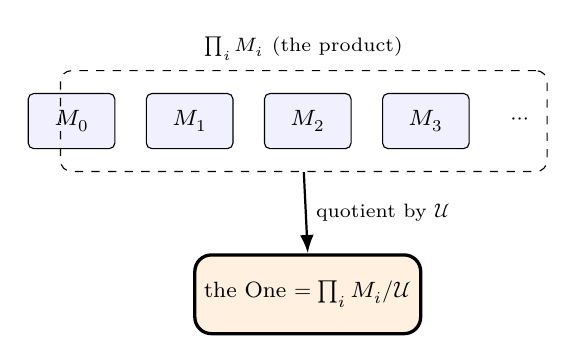
\begin{tikzpicture}[
  >=Latex, every node/.style={font=\footnotesize},
  fac/.style={draw, rounded corners=2pt, fill=blue!6, minimum width=11mm,
              minimum height=7mm},
  one/.style={draw, very thick, rounded corners=6pt, fill=orange!12,
              minimum width=24mm, minimum height=10mm, align=center}
]
  \foreach \x/\lab in {0/$M_0$,1.5/$M_1$,3/$M_2$,4.5/$M_3$} {
    \node[fac] (m\lab) at (\x,0) {\lab};
  }
  \node at (5.7,0) {$\cdots$};
  \node[draw, dashed, rounded corners, fit={(0,-0.5)(5.9,0.5)}, inner sep=4pt,
        label=above:{\scriptsize $\uprod_i M_i$ (the product)}] (prod) {};
  \node[one] (one) at (3,-2.2) {the One $=\uprod_i M_i / \Uf$};
  \draw[->, thick] (prod.south) -- (one.north)
       node[midway, right, font=\scriptsize]{quotient by $\Uf$};
\end{tikzpicture}
\caption{Product-mod-ultrafilter (D2). The finite factors $M_i$ are coordinates;
the One is their product collapsed by the ultrafilter's notion of ``almost all.''
Nothing finite is fundamental---each $M_i$ is a projection.}
\label{fig:prod}
\end{figure}

\subsection{A second home: adjoint modalities and the structural reading}
\label{sec:adjoint}

The ultraproduct is one formal home; there is a second, complementary one in
type theory, and it answers the natural question ``if the finite is a projection,
what \emph{kind} of map is the projection?'' The answer is: an \emph{adjoint
modality}. In Shulman's cohesive and multimodal adjoint type theories, a continuous
(``cohesive'') ground carries a discrete modality $\flat$ that is part of an
adjoint string---shape $\int\dashv\flat\dashv\sharp$ codiscrete---so that the
\emph{discrete, finitary} layer is \emph{recovered from} the continuous one by a
modality with an adjoint, not posited independently
\cite{Shulman2018Cohesive, GratzerMTT2020, ShulmanMATT2023}. This is the precise
type-theoretic form of the intuition that finitary structure is a forgetful/adjoint
shadow of a richer continuum, and it is the modal core a
multimodal type theory for MeTTa would be built to host.

The same move dissolves the ``atom'' worry about the number $1$. In a structural
foundation---an elementary topos, or homotopy type theory---there are no primitive
elements at all; $1$ is the \emph{terminal object}, characterized purely by a
universal property (a unique map from every object), and ``elements'' of $X$ are
maps $1\to X$, derived rather than given \cite{MacLaneMoerdijk1992, HoTTBook}. The
finitary is relational all the way down: ``$1$ as an equivalence class of all
objectifiable systems'' is exactly ``$1$ as the object every count factors
through.''

\begin{remark}[the Axiom of Para-Infinity]
\label{rem:para}
There is a candid epistemic companion to the metaphysical thesis: we possess
\emph{positive evidence for both} ``the Universe is finite'' and ``the Universe is
infinite,'' so a disciplined reasoner should carry both. This Axiom of
Para-Infinity is not a hedge but an instance of Section~\ref{sec:teethB}: it places
a \emph{credal interval} on the finiteness question itself. Where a precise
metaphysics would collapse to one principal verdict, Para-Infinity keeps the free
ensemble, and the open-world width is the honest report of our uncertainty about the
very thing the thesis is about.
\end{remark}

\section{Ultrainfinitism formalized}
\label{sec:formal}

We can now state the reading precisely, and we index it honestly: there is no
canonical free ultrafilter, so there is no single absolute ``One.'' Given a family
$M=(M_i)_{i\in I}$ and a free ultrafilter $\Uf$ on $I$, the \emph{relative One} is
the ultraproduct
\[
  \textstyle
  \mathrm{One}_{(M,\Uf)} \;:=\; \bigl(\uprod_i M_i\bigr)/\Uf .
\]
We write $\limstar := \mathrm{One}_{(M,\code{hyperfilter})}$ for the canonical-cofinite
choice and keep ``the One'' as evocative shorthand once the indexing is in place.
What deserves the definite article is not any one $\mathrm{One}_{(M,\Uf)}$ but the
\emph{invariant}: by {\L}o\'s (Theorem~\ref{thm:los}), the \emph{first-order theory}
$\mathrm{Th}(\mathrm{One}_{(M,\Uf)})$ depends only on the ``$\Uf$-almost-all'' filter
and is preserved under every coordinate permutation; the dependence on \emph{which}
free $\Uf$ is exactly the perspectival latitude that Section~\ref{sec:teethB}
measures as credal width. Singular language tracks the invariant; the indexed
object tracks the choice.

\begin{definition}[envisioned reading]
\label{def:reading}
A first-order property $\varphi$ is \emph{ultrainfinitistically true} of the family
when it holds in the One, $\limstar\models\varphi$. A truth-value assessment is
\emph{precise} when it is taken along a principal ultrafilter (a single
coordinate) and \emph{open} when it is taken along a free ultrafilter (the One,
with its tail-relative verdict).
\end{definition}

Three comments fix the status of Definition~\ref{def:reading}. First, ``nothing
finite truly exists'' is, mathematically, the observation that \emph{no principal
ultrafilter is canonical}: there is no privileged coordinate, only the choice of a
perspective; the free One is what is invariant under that choice, and {\L}o\'s
(Theorem~\ref{thm:los}) is what lets a perspective transfer truth to and from it.
Second, Definition~\ref{def:reading} is now \emph{built}: the formal core
(\lpath{Mettapedia/Logic/Metaphysics/UltrainfinitismCore.lean}, sorry-free and
axiom-clean) defines \code{UltraTrue} ($=$ \emph{ultrainfinitistly true}: truth from
the perspective of an ultrafilter, the verdict of the relative One) together with
\code{PreciseFamily}/\code{OpenFamily}, and proves the small canonical lemmas this
section promises: \emph{principal collapse} (\code{ultraTrue\_pure}: from a principal
perspective, ultrafilter truth is truth at the generating coordinate),
\emph{invariance} (\code{ultraTrue\_map}: re-coordinatizing the index
re-coordinatizes the One and changes nothing else), the \emph{envelope theorems}
(\code{ultraTrue\_all\_iff}/\code{\_exists\_iff}: the lower/upper envelope over all
perspectives is the universal/existential coordinate verdict), the \emph{dial
dichotomy} (\code{openFamily\_iff\_not\_precise}: a family is open exactly when it is
not precise, i.e.\ exactly when the coordinates genuinely disagree), the
\emph{free/principal separation} (\code{hyperfilter\_pure\_disagree}: the free One
affirms what a finite coordinate-shadow denies), and the {\L}o\'s
\emph{transfer} in wrapper form (\code{ultraTrue\_iff\_uprod}, with
\code{ultrapower\_elementary}: a structure is elementarily equivalent to every
ultrapower of itself). Third---in
the interest of honesty---the file currently named
\lpath{Mettapedia/Hyperseed/Ultrainfinitism.lean} is \emph{not} this construction:
it is a budget-bounded ``perspective'' shell (signal classes, effort costs,
availability regions) that models a \emph{finitary observer's access}, the
\emph{dual} pole of the present idea, and is a misnomer to be superseded by the
ultraproduct reading. We flag this rather than paper over it.

\section{Three theorems with teeth}
\label{sec:teeth}

Ultrainfinitism would be mere poetry if it floated free of proof. It does not.
Three already-proved, sorry-free fragments of the Mettapedia development are
precisely the principal/free, finite/infinite picture in action.

\subsection{(A) Conjecturing in the limit}
\label{sec:teethA}

A universal mathematical conjecture---``every finite structure of this kind
satisfies $\varphi$''---is, on the ultrainfinitist reading, a claim about the One.
By {\L}o\'s (Theorem~\ref{thm:los}), $\limstar\models\varphi$ iff $\varphi$ holds
on an ultrafilter-large set of finite coordinates. This yields a clean trichotomy
for an automated conjecturer that enumerates finite witnesses (loops, groups,
graphs) by some size parameter:
\begin{itemize}
\item \emph{proved}: $\varphi$ holds at \emph{every} coordinate, hence in every
ultraproduct (equational/first-order transfer);
\item \emph{refuted}: $\varphi$ fails \emph{cofinally}, so a counterexample exits
the closure and $\varphi$ fails for ultrafilter-many coordinates;
\item \emph{open}: the truth of $\varphi$ is \emph{ultrafilter-ambiguous in the
tail}---it holds on one infinite set of sizes and fails on another.
\end{itemize}
The inductive leap from ``all sampled sizes'' to ``all sizes'' is thus not a
hand-wave but the transfer principle: it asks whether the sampled pattern survives
to the One.

Our loop-theory conjecturer exhibits the three regimes concretely. Enumerating
finite loops by order and mining equational implications, it certifies some
candidates as theorems (transfer to every order, hence to the One), and it watches
others break \emph{cofinally}: the implication ``Moufang $\Rightarrow$
associative'' holds through order eleven and then fails at order twelve---the
smallest non-associative Moufang loop---so it fails for ultrafilter-many orders and
is refuted in the One. The genuinely interesting residue is the third regime: a
hardened candidate such as ``flexible and left-alternative $\Rightarrow$
left-inverse-property'' survives every order the prover can reach, leaving its
status in the One open---an ultrafilter-ambiguous tail awaiting either a transfer
proof or a cofinal counterexample. These are not three labels we impose; they are
the three ways a sampled pattern can relate to the limit object.

Our concept-formation layer already exhibits the elementary form of this gap. In
the formal-concept setting, the closure of a premise over a \emph{sampled}
population can strictly exceed its closure over the \emph{full} population, and the
difference is a witnessable object. The control example is deliberately homely:
over the two-element sample $\{\text{robin}, \text{bat}\}$, the implication
``winged $\Rightarrow$ flies'' \emph{holds}; over the full context (which contains
the penguin) it \emph{fails}.

\begin{theorem}[sampled-vs-full frontier; \code{flies\_mem\_winged\_scrutability\_frontier}, \lpath{LoopConjectureScrutability.lean:397}]
\label{thm:flies}
\[
\text{flies}\in \mathrm{sampledClosure}(\{\text{robin},\text{bat}\},\,\{\text{winged}\})
\quad\text{and}\quad
\text{flies}\notin \mathrm{fullClosure}(\{\text{winged}\}).
\]
\end{theorem}

This is exactly an ultrainfinitist tail phenomenon in miniature: a truth of the
finite shadow that the larger (eventually infinite) context overturns. The
\emph{credal} version makes the imprecision quantitative, and it is the subject of
(B).

\subsection{(B) Precise $=$ principal, imprecise $=$ free}
\label{sec:teethB}

Index a family of admissible perspectives by ``gates'' $\Gamma$. Each gate yields a
sharp verdict; the ensemble yields an interval. Two theorems make the dial exact.

First, imprecision \emph{is} disagreement among perspectives. The credal width
collapses to zero exactly when all gates agree---i.e.\ exactly when the assessment
is, in effect, principal (a single coordinate's verdict suffices):

\begin{theorem}[precision $=$ unanimity; \code{inheritanceCredalWidth\_eq\_zero\_iff}, \lpath{ExtensionalIntensionalDivergence.lean:488}]
\label{thm:width}
\[
\mathrm{credalWidth}_\Gamma(\text{sub},\text{super})=0
\;\Longleftrightarrow\;
\forall\,g,h\in\Gamma:\;
\mathrm{strength}_{g}(\text{sub},\text{super})=\mathrm{strength}_{h}(\text{sub},\text{super}).
\]
\end{theorem}

Second, the interval endpoints are not ad hoc: the lower and upper inheritance
strengths are the \emph{greatest lower bound} and \emph{least upper bound} of the
ensemble of per-gate strengths---the Walley lower and upper envelopes of the
induced credal set \cite{Walley1991, Walley1996BagOfMarbles}:

\begin{theorem}[Walley envelope; \code{lowerInheritanceStrength\_isGLB} / \code{upperInheritanceStrength\_isLUB}, \lpath{InheritanceIntegration.lean:125,139}]
\label{thm:env}
$\mathrm{lower}_\Gamma$ is $\operatorname{IsGLB}$ and $\mathrm{upper}_\Gamma$ is
$\operatorname{IsLUB}$ of $\{\,\mathrm{strength}_g : g\in\Gamma\,\}$.
\end{theorem}

The ultrainfinitist reading is then forced. A \emph{principal} perspective collapses
the credal set to a point---a precise probability, the special case. A \emph{free}
perspective keeps the whole ensemble and reports the envelope---an interval whose
width measures how far the perspectives spread, i.e.\ the tail-ambiguity of the
One. Precision is the principal-ultrafilter shadow of an irreducibly imprecise,
free-ultrafilter ground. Concept formation shows the same structure with a binary
outcome: the credal scrutability gap (concepts formed under some gate but not all)
carries envelope width exactly $1$ on the gap and $0$ off it.

\begin{theorem}[gap $=$ unit width; \code{globalEnvelopeWidth\_\ldots\_eq\_indicator\_credalScrutabilityGap}, \lpath{LoopConjectureScrutability.lean:330}]
\label{thm:gap}
$\mathrm{credalScrutabilityGap}=\mathrm{upperFamily}\setminus\mathrm{lowerFamily}$,
and the global envelope width of the concept-formation gamble is the indicator of
this gap.
\end{theorem}

\begin{figure}[H]
\centering
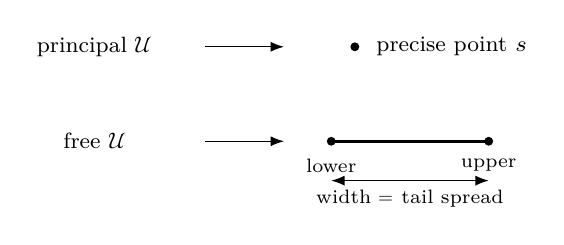
\begin{tikzpicture}[
  >=Latex, every node/.style={font=\footnotesize}
]
  % principal -> point
  \node (p) at (0,0.6) {principal $\Uf$};
  \draw[->] (1.4,0.6) -- (2.4,0.6);
  \fill (3.3,0.6) circle (1.6pt);
  \node[right] at (3.45,0.6) {precise point $s$};
  % free -> interval
  \node (f) at (0,-0.6) {free $\Uf$};
  \draw[->] (1.4,-0.6) -- (2.4,-0.6);
  \draw[very thick] (3.0,-0.6) -- (5.0,-0.6);
  \fill (3.0,-0.6) circle (1.6pt); \fill (5.0,-0.6) circle (1.6pt);
  \node[below] at (3.0,-0.7) {\scriptsize lower};
  \node[below] at (5.0,-0.7) {\scriptsize upper};
  \draw[<->] (3.0,-1.1) -- (5.0,-1.1)
        node[midway, below, font=\scriptsize] {width $=$ tail spread};
\end{tikzpicture}
\caption{The precise/credal dial (D3). A principal ultrafilter collapses the credal
set to a precise point (Theorem~\ref{thm:width}); a free ultrafilter reports the
Walley envelope (Theorem~\ref{thm:env}), whose width measures perspective spread.}
\label{fig:credaldial}
\end{figure}

\subsection{(C) Infinite-primary de Finetti}
\label{sec:teethC}

The third fragment is the probabilistic heart, and it shows ultrainfinitism not as
a reinterpretation but as a \emph{method}. De~Finetti's theorem concerns infinite
exchangeable sequences: an exchangeable law on $\{0,1\}^{\N}$ is a mixture of
i.i.d.\ Bernoulli laws, $\nu=\int_{[0,1]}\mathrm{Bernoulli}(\theta)^{\otimes\N}\,
d\mu(\theta)$ \cite{definetti1937, deFinetti1974}. In our development the mixture
is a first-class object,
\begin{center}
\code{structure BernoulliMixture} with a \code{mixingMeasure} on $[0,1]$
\quad(\lpath{Logic/DeFinetti.lean:130}),
\end{center}
and the exchangeable, count-only character of its finite marginals is proved
(\code{infiniteExchangeable\_same\_counts\_same\_prob},
\lpath{DeFinetti.lean:203}); the unique latent measure is exported stably
(\lpath{CategoryTheory/DeFinettiStableExports.lean:31}).

The ultrainfinitist point is about \emph{construction order}. The naive impulse is
to build the global object by \emph{extending} finite-prefix data outward to the
infinite sequence---and this is exactly where such constructions stall, on the gap
between finitely-specified prefix laws and a coherent law on the full product.
Ultrainfinitism says: do not extend the finite; \emph{the infinite is primary}.
Construct $\nu$ on $\{0,1\}^{\N}$ first---as a genuine infinite-product measure,
the probabilistic sibling of the ultraproduct---and recover each finite-prefix law
as a \emph{projection} (a marginal), not as a building block. The ``raw versus
finite'' gap dissolves because the arrow was pointing the wrong way: the One
measure is the datum; the finite prefixes are its principal-ultrafilter shadows.

\begin{figure}[H]
\centering
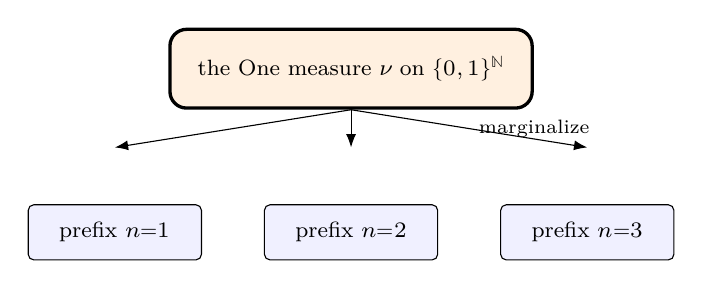
\begin{tikzpicture}[
  >=Latex, every node/.style={font=\footnotesize}
]
  \node[draw, very thick, rounded corners=6pt, fill=orange!12, minimum width=46mm,
        minimum height=10mm, align=center] (nu)
        {the One measure $\nu$ on $\{0,1\}^{\N}$};
  \foreach \x/\lab in {-3/{prefix $n{=}1$},0/{prefix $n{=}2$},3/{prefix $n{=}3$}} {
    \node[draw, rounded corners=2pt, fill=blue!6, minimum width=22mm,
          minimum height=7mm, below=12mm of nu, xshift=\x cm] (p\lab) {\lab};
  }
  \draw[->] (nu.south) -- (-3,-1.0) node[midway,left,font=\scriptsize]{};
  \draw[->] (nu.south) -- (0,-1.0);
  \draw[->] (nu.south) -- (3,-1.0) node[midway,right,font=\scriptsize]{marginalize};
\end{tikzpicture}
\caption{Infinite-primary de~Finetti (D4). The infinite mixture $\nu$ is the datum;
finite-prefix laws are downward projections (marginals), not building blocks.}
\label{fig:definetti}
\end{figure}

\section{Native homes, and a worked prototype: gunky mereology}
\label{sec:gunk}

The ultraproduct core says \emph{what} the finite is (a principal shadow) but not
\emph{where} an infinite-native universe should live---a foundation in which ``no
finitary elements'' is built in rather than asserted against a finitary scaffolding
(Section~\ref{sec:objections}). Four candidate homes recur; we score them and then
prototype the most tractable.

\begin{table}[H]
\centering\small
\begin{tabular}{@{}lccccc@{}}
\toprule
Native home & no empty & no atomic & observer- & constructive & Lean \\
 & individual & base & relativity & friendly & feasibility \\
\midrule
Universal-set (NF/NFU) & no & partial & weak & no & \emph{Con} formalized\footnotemark \\
Non-well-founded (AFA) & no & yes & partial & partial & core in mathlib \\
\textbf{Atomless gunk} & \textbf{yes} & \textbf{yes} & \textbf{yes} & yes & \textbf{prototyped here} \\
Structural (topos/HoTT) & yes & yes & yes & yes & topos in mathlib; HoTT elsewhere \\
\bottomrule
\end{tabular}
\caption{The native-foundation scorecard. Gunk most directly answers the
empty-set/atom issue while staying closest to the phenomenology, and it is the one we
prototype below.}
\label{tab:homes}
\end{table}
\footnotetext{The consistency of New Foundations is verified in Lean~4 (Holmes--Wilshaw),
so the universal-set home is now machine-checked at the consistency level
\cite{HolmesWilshawNF}; it remains a heavyweight, separate development.}

\subsection{Gunk forces the infinite}
\label{sec:gunk-core}

A \emph{gunky} (atomless) order is one in which every individual is properly
divisible---the mereological form of ``you can always look deeper.''

\begin{definition}[gunky order]
\label{def:gunky}
A bounded order $(\alpha,\le,\bot)$ is \emph{gunky} when every non-bottom element has
a proper non-bottom part: $\forall a\neq\bot,\ \exists b\neq\bot,\ b<a$. Equivalently,
$\alpha$ has \emph{no atoms}.
\end{definition}

The load-bearing fact---and the formal counterpart of Bridge
Principle~\ref{prin:bridge1} feeding into Principle~\ref{prin:bridge2}---is that gunk
\emph{forces} infinitude. The finite cannot be gunky.

\begin{theorem}[gunk $\Rightarrow$ infinite; \code{infinite\_of\_isGunky}, \lpath{GunkyMereology.lean}]
\label{thm:gunk-inf}
Every gunky order with more than one element is infinite. Iterating ``take a proper
non-bottom part'' produces a strictly descending sequence $a_0>a_1>a_2>\cdots$, an
injection $\N\hookrightarrow\alpha$.
\end{theorem}

Gunk is not vacuous, and it is not universal---we give both poles. The two
genuinely two-dimensional algebra witnesses are the ones one wants:

\begin{theorem}[two gunky algebras; \code{isGunky\_clopens\_cantor}, \code{isGunky\_opens\_real}]
\label{thm:gunk-witness}
The Boolean algebra of \emph{clopen subsets of Cantor space} $2^{\N}$ is gunky (a
nonempty clopen splits: fix one more coordinate), and the frame---complete Heyting
algebra---of \emph{open regions of $\R$} is gunky (shrink the radius). The non-negative
reals furnish the linear case (every magnitude is halvable), while a two-valued algebra
is the paradigm non-gunky one (\code{not\_isGunky\_bool}): its top is an atom.
\end{theorem}

All of Theorems~\ref{thm:gunk-inf}--\ref{thm:gunk-witness} are formalized in Lean~4,
sorry-free and with only the standard axioms; the statements are transcribed in
Appendix~\ref{app:lean}. Spatial regions of the continuum, and clopen cylinders of
Cantor space, are thus genuine atomless universes---no empty individual is forced, no
minimal part exists, and the universe is provably infinite.

\subsection{Stone duality: atoms are the principal-ultrafilter points}
\label{sec:stone}

Gunk connects to the paper's central dial not by analogy but by Stone duality, which
is the place the principal/free story comes closest to a representation theorem
(answering, in part, the critique that the dial is only an organizing principle).

\begin{theorem}[Stone duality: atomless $\Leftrightarrow$ perfect]
\label{prop:stone}
Let $B$ be a Boolean algebra and $S(B)$ its Stone space, realized as the prime spectrum
of the Boolean ring of $B$. Then there is an order isomorphism
$B\;\cong\;\mathrm{Clopens}\bigl(S(B)\bigr)$ (the \emph{Stone representation}: $B$ is the
clopen algebra of its Stone space), $S(B)$ is compact, Hausdorff and totally separated,
and the \emph{atoms} of $B$ correspond exactly to the \emph{isolated points} of
$S(B)$---which, in the Stone topology, are exactly the \emph{principal} ultrafilters.
Hence
\[
  B \text{ is atomless (gunky)}
  \quad\Longleftrightarrow\quad
  S(B) \text{ is \emph{perfect} (has no isolated point).}
\]
In the powerset $B=\mathcal P(X)$ the atoms are the singletons $\{x\}$, i.e.\ the
supports of the principal ultrafilters $\mathrm{pure}\,x$ (\code{isAtom\_set\_singleton});
so $\mathcal P(X)$ is never gunky for inhabited $X$ (\code{not\_isGunky\_set}).
\end{theorem}

This is now formalized \emph{in full generality}---for an arbitrary Boolean algebra,
not merely the powerset or Cantor instances---sorry-free and axiom-clean:
\code{stoneRepr} (the order isomorphism) and \code{isGunky\_iff\_perfect\_stoneSpace}
(the equivalence) in \lpath{Mettapedia/Logic/StoneGunkDuality.lean}; the bottleneck, that
the Boolean-ring spectrum is Hausdorff, is proved from the complementary clopens
$\mathrm{basicOpen}\,e$ and $\mathrm{basicOpen}\,(1-e)$. Read against the dial: an atom is
precisely a \emph{principal-ultrafilter} point, so ``gunky'' is exactly ``no finitary,
principal-shadow point stands alone.'' The finite (isolated/principal) is never
fundamental; an atomless universe has only free, limit points---the relative Ones of
Section~\ref{sec:formal}. The slogan ``finite $=$ principal shadow'' is thereby upgraded
to the dual \emph{theorem} ``finite atom $=$ isolated point.''

\subsection{A model of ultrainfinitism}
\label{sec:model}

We can now say what a \emph{model} of the thesis looks like---a structure in which it
holds, in the sense in which one builds a model of a set theory.

\begin{definition}[gunky--Stone model]
\label{def:model}
A \emph{gunky--Stone model} is a pair $\langle B,\,S(B)\rangle$ with $B$ an atomless
Boolean (or Heyting) algebra and $S(B)$ its Stone space. Reality is $B$: every
individual is infinitely divisible (gunk), and the universe is infinite
(Theorem~\ref{thm:gunk-inf}). A ``finite world a perspective lives in'' is a point of
$S(B)$---a choice of ultrafilter; but since $B$ is atomless, $S(B)$ is perfect
(Theorem~\ref{prop:stone}), so \emph{no such point is isolated}: every finitary
reading is a limit of others. That is the Law of Oneish, modelled.
\end{definition}

The Cantor witness is the self-dual jewel: $S\bigl(\mathrm{Clopens}(2^{\N})\bigr)=2^{\N}$
itself, which is perfect. The gunky algebra and its perfect point-space are two faces
of one object, and ``no isolated point'' is ``no finite atom.'' We have built the
universe (two atomless witnesses), the no-atom axiom (gunk), the infinitude theorem,
the Stone representation $B\cong\mathrm{Clopens}(S(B))$, and---now in full
generality---the classical equivalence $\text{atomless}\Leftrightarrow\text{perfect}$
(Theorem~\ref{prop:stone}). The point-layer's {\L}o\'s transfer is now also in place:
the formal core (Section~\ref{sec:formal}) provides
\code{ultraTrue\_iff\_uprod}---ultrainfinitist truth of a first-order sentence along a
family \emph{is} truth in the ultraproduct---and its constant-family corollary
\code{ultrapower\_elementary}: a structure is elementarily equivalent to every
ultrapower of itself, so $B$ and the Ones built over it validate exactly the same
first-order truths. One caveat is layer-honesty, learned from the concept-formation
side: the atomic/gunky dial must always be indexed to \emph{which} algebra carries
it---a derived algebra (a frontier, a quotient, a concept state) may sit at a
different pole than its base. The transfer lemmas (\code{isGunky\_congr},
\code{isGunky\_Iic}, \code{perfectSpace\_stoneSpace\_congr}) exist precisely to move
the dial to the right carrier.

\paragraph{The dial, welded.} The faces of the dial are now not merely parallel but
\emph{provably one object}, in three welds. (i)~\emph{Algebra--space}: the semantic
ultrafilter-sets of the second-order layer are exactly the points of the Stone space
(\code{ultraSetEquivStonePoint}), having a least element is being an isolated point
(\code{hasLeast\_iff\_isOpen\_singleton}), and the two previously parallel chains close
into one circle: the free-ultrafilter axiom holds iff the Stone space is perfect
(\code{sat\_freeUFAx\_iff\_perfect\_stoneSpace})---free axiom $\Leftrightarrow$ no
principal ultrafilter $\Leftrightarrow$ no atom $\Leftrightarrow$ no isolated point
$\Leftrightarrow$ perfect. (ii)~\emph{Index--algebra}: relative truth
$\mathrm{UltraTrue}$ is evaluation of the verdict-set at a Stone point of the powerset
algebra (\code{ultraTrue\_iff\_mem}); a principal perspective is evaluation at an
\emph{atom} (\code{ultraTrue\_pure\_iff\_atom\_le}); precision is degeneracy to
$\bot$/$\top$ and openness is residence in the frontier
(\code{preciseFamily\_iff\_degenerate}, \code{openFamily\_iff\_nontrivial\_proper}).
(iii)~\emph{Inference--metaphysics}: the credal open-world/that's-all predicates of the
concept-formation layer are \emph{equal} to the perspectival dial---a concept is
open-world iff its gate-verdict family is an open family, that's-all iff precise
(\code{openWorldConcept\_iff\_openFamily}, \code{thatsAllConcept\_iff\_preciseFamily}).
And the principal-shadow slogan is now a theorem-\emph{pair}: a finite frontier is
provably atomic (\code{not\_isGunky\_of\_finite}), and a finite perspective-space has
only principal points (\code{ultraTrue\_of\_finite})---gunk and free perspectives both
live only in the limit, exactly as the thesis demands. At the inference layer the dial
now also separates the reasoning modes themselves: under that's-all premises induction
is gate-invariantly precise, while abduction strengths provably \emph{vary} across
gates once the explanatory edge is open-world and nondegenerate---Peirce's intuition
that explanation-seeking lives in the open world, as an exact statement.

\subsection{Formal philosophy: gunk versus mereological nihilism}
\label{sec:sider}

The atomless/atomic contrast has a sharp philosophical edge. \emph{Mereological
nihilism} holds that there are no composite objects: every object is a mereological
\emph{simple} (an atom). Sider \cite{Sider1993} argues against it from the mere
\emph{possibility} of gunk: (1)~nihilism is non-contingent (necessarily true or
necessarily false); (2)~gunk is metaphysically possible; (3)~if gunk is possible,
nihilism is not necessary; (4)~therefore nihilism is necessarily false.

We formalize the argument with the standard semantic reading of metaphysical modality:
a \emph{world} is a parthood structure (a bounded order on $\geq 2$ individuals), with
$\Box P := \forall W,\,P\,W$ and $\Diamond P := \exists W,\,P\,W$ (the universal, $S5$
frame). \emph{Sider's nihilism} at a world says ``every object is a simple,''
$\forall a\neq\bot,\ \mathrm{IsAtom}\,a$ (\code{SiderNihilism}); ``gunky'' reuses
\code{IsGunky}. Two halves are then \emph{theorems}, sorry-free and axiom-clean, in
\lpath{Mettapedia/Logic/Metaphysics/SiderNihilism.lean}:
\begin{itemize}
\item \textbf{The argument is valid, and premises 2--3 are proved.} Gunk is possible
  (witnessed by the continuum, \code{possible\_gunk}), and a gunky world is never a
  nihilist world (\code{gunky\_not\_siderNihilism}: gunk means \emph{no} atoms, nihilism
  requires \emph{all} simples). Hence \code{siders\_argument}:
  $\mathrm{NonContingent}(N)\Rightarrow\Box\neg N$---granting premise~1, nihilism is
  necessarily false.
\item \textbf{But premise~1 fails in the unrestricted logical space of mereologies}
  (\code{not\_nonContingent\_siderNihilism}): there is a gunky world \emph{and} a nihilist
  world (a two-element order), so neither nihilism nor its negation is necessary. Nihilism
  is genuinely \emph{contingent} across parthood structures
  (\code{siderNihilism\_contingent}).
\end{itemize}

The formalization thus vindicates Sider's premises 2--3 as theorems and localizes the
whole dispute on premise~1: the argument is \emph{valid} but sound only under the
metaphysical posit that restricts the space of worlds so nihilism becomes non-contingent.
Via Theorem~\ref{prop:stone} this is a Stone-dual picture: nihilism is the
\emph{discrete} pole (every point of $S(B)$ isolated), gunk the \emph{perfect} pole
(no isolated point), and both poles are realized---which is precisely why premise~1 is not
a logical truth. The ultrainfinitist takes the gunky/perfect pole as the real one, and
\code{infinite\_of\_isGunky} with Theorem~\ref{prop:stone} say why it is the anti-nihilist
limit: no isolated point, no finite simple, the universe infinite.

\section{Philosophical ramifications}
\label{sec:philo}

\paragraph{Process before substance.} If the finite is an act of distinction rather
than a stock of given things, then \emph{becoming} is prior to \emph{being}---a
thesis with a long process-philosophical lineage (Whitehead) and a contemporary
operational echo in the Hyperseed ontology, where ``process'' and ``becoming'' are
primitive and a transition phase is explicitly a zone in which the
A/B distinction blurs \cite{Whitehead1929, GoertzelHyperseed}. The ultraproduct
gives this teeth: the finite coordinate is the snapshot, the One is the ongoing
whole, and {\L}o\'s says which snapshot-truths are truths of the whole.

\paragraph{Distinction is observer-relative.} The choice of principal ultrafilter
\emph{is} the choice of which coordinate to call ``the world.'' This is the formal
residue of the phenomenological point of Section~\ref{sec:prologue}: a finite
object is a reading, and a reading presupposes a reader---a perspective that draws
the distinction. Goertzel's constructive-nonstandard concept makes the dual
movement explicit from the finite side: a finite distinguishing system, with a
distinguishability relation $\mathrm{DS}$ and a resolution band $[\min_S,\max_S]$,
calls \emph{potentially infinite} whatever exceeds its resolution
\cite{GoertzelHyperseed}. That is the coordinate's view looking \emph{up} at the
One; ultrainfinitism is the One's view looking \emph{down} and projecting
finitudes. The two are the principal and free poles of a single ultrafilter
lattice, and {\L}o\'s is the bridge between them.

\paragraph{The continuum as ground.} Reading discreteness as emergence rather than
foundation aligns ultrainfinitism with the field-theoretic picture in physics and
with the internal-language view of topos theory, in which the locally-discrete and
the globally-continuous are two faces of one sheaf-theoretic structure
\cite{MacLaneMoerdijk1992}. The neutral-monist intuition---that the apparent
plurality of things is the differentiation of one underlying stuff
\cite{Russell1914}---is, on this reading, the Law of Oneish stated in the key of
metaphysics rather than model theory.

A caution, in the same spirit of honesty as Section~\ref{sec:formal}: of the
thinkers invoked here, only the operational, locally-grounded fragments enter our
formal claims. Whitehead, Russell, and Carnap are cited as genuine intellectual
lineage, not as authorities whose theses we have formalized.

\section{Practical ramifications and applications}
\label{sec:practical}

\paragraph{Conjecture confidence as tail behaviour.} Section~\ref{sec:teethA}
turns an automated conjecturer's verdicts into statements about the One. A practical
ranking follows: an open conjecture's credal width
(Theorems~\ref{thm:width}--\ref{thm:gap}) is a measure of \emph{tail ambiguity}, so
conjectures whose sampled support is robust across perspectives (small width) are
better bets than those that hold only on a perspective-dependent set of sizes. This
is a principled, proof-anchored alternative to ranking by raw sample frequency.

\paragraph{Build the infinite first (imprecise Bayes).} Section~\ref{sec:teethC} is
a constructive recommendation, not only a reinterpretation: when a global
stochastic process is wanted from a consistent family of finite-dimensional laws,
construct the infinite-product/mixture object and read off finite marginals,
rather than struggling to extend finite data outward. The imprecise version is the
\emph{imprecise Dirichlet} stance \cite{Walley1996BagOfMarbles}: carry a credal set
of mixing measures, and let the Walley envelope (Theorem~\ref{thm:env}) report the
free-ultrafilter spread; precision is recovered only by the principal collapse to a
single mixing measure.

\paragraph{Scale-relativity in physics and learning (a conjectural prompt).} We mark
this lane explicitly as suggestive alignment rather than a proved anchor. The
renormalization-group picture in physics and the continuum limits of large neural
networks \emph{appear} to share the ultrainfinitist shape: the ``physical'' or
``trained'' object reads as a scale-relative projection of an underlying continuum,
with the finite, discretized model as the coordinate one happens to compute in. That
suggests reading finite-size artefacts (lattice spacing, network width) as perspective
parameters rather than approximations to apologize for. We offer this as a research
prompt for a future toy model, not as evidence on the level of
Sections~\ref{sec:teeth}--\ref{sec:gunk}; the formal core should be hardened first.

\section{Objections and replies}
\label{sec:objections}

A thesis worth holding is worth attacking. We state the strongest objections we
know and answer them.

\paragraph{``This is just nonstandard analysis dressed in metaphysics.''}
Nonstandard analysis is a tool; ultrainfinitism is a claim about \emph{priority}
and a \emph{unification}. The tool says infinite and infinitesimal elements can be
constructed and reasoned with via ultrapowers; the thesis says the infinite
construction is the primary thing and the finite is its projection, and---this is
the content beyond NSA---that \emph{the same dial} governs conjecture
(Section~\ref{sec:teethA}), credence (Section~\ref{sec:teethB}), and concept
formation (Theorem~\ref{thm:gap}). What NSA leaves as a technique for analysis,
ultrainfinitism reads as a single construction principle across three activities
we usually keep apart.

\paragraph{``Free ultrafilters are not canonical---so `the One' is ill-defined.''}
There are many free ultrafilters and (under the usual axioms) no way to name one;
the ultraproduct depends on the choice. We embrace this rather than resist it. The
\emph{absence} of a privileged coordinate is exactly Principle~\ref{prin:ui}: no
finite shadow is the world. And the residual dependence on \emph{which} free
ultrafilter is not a defect but the formal seat of imprecision: it is the
tail-ambiguity that Theorem~\ref{thm:width} measures as nonzero credal width.
What is invariant---the first-order theory transferred by {\L}o\'s, the envelope of
verdicts---is what ultrainfinitism calls real; what varies with the ultrafilter is
exactly what it calls perspectival. The objection, pressed, becomes the theory.

\paragraph{``Skolem and L\"owenheim\,--\,Skolem show the infinite is not even pinned
down.''} Correct, and unneeded. Ultrainfinitism does not require a unique infinite
model, a categorical theory, or a settled cardinality. It requires only that the
infinite be \emph{primary} and the finite a projection, with transfer as the
invariant bridge. Non-categoricity is, again, perspectival latitude---more One than
any coordinate can pin, which is the expected shape of a ground that exceeds its
shadows.

\paragraph{``Then drop first-order logic: full second-order semantics restores
categoricity, and your latitude evaporates.''} The strongest form of the previous
objection, and the most instructive. With \emph{standard} (full) second-order
semantics, Dedekind pins $\N$, Huntington pins $\R$, and Zermelo quasi-pins the
set universe; L\"owenheim--Skolem is a first-order artifact. But by Lindstr\"om's
theorem \cite{Lindstrom1969}, the price is mandatory: any logic with compactness
and downward L\"owenheim--Skolem is no stronger than first-order, so full
second-order logic forfeits completeness, compactness, and any effective proof
calculus---it pins the model from a vantage no finite agent occupies (it
``decides'' the continuum hypothesis without telling anyone how). Henkin's general
models \cite{Henkin1950} restore the finitary virtues for the \emph{same} syntax,
and thereby re-import the latitude; Farmer counts this dual semantics among simple
type theory's virtues \cite{Farmer2008}. Our reply: the standard/Henkin switch
\emph{is} the principal/free dial, reappearing at the level of semantics itself.
Full semantics is the ground-side face (categorical, no effective access); the
Henkin family of general models is the shadow-side face (effective, many
perspectives); and full-semantics categoricity is \emph{borrowed determinacy}---%
$\N$ is pinned only relative to a metatheoretic totality of ``all subsets'' that is
itself only quasi-categorical. The latitude is not eliminated but promoted one
level, which is the thesis exhibiting itself. This reply is now formalized: one
monadic second-order syntax with both semantics, in which the ultrainfinitist core
theory---gunk, nontriviality, and the genuinely second-order axiom \emph{every
ultrafilter is free}---is satisfiable under the standard reading and over
\emph{every} Henkin family whatsoever \emph{by the same gunky witness}, the Cantor
clopen algebra (\code{T\_UI\_satisfiable\_standard},
\code{T\_UI\_satisfiable\_all\_henkin}); the free-ultrafilter axiom is provably
\emph{equivalent} to first-order atomlessness over standard semantics
(\code{sat\_freeUFAx\_iff\_isGunky}---the Stone dictionary internalized into the
object language) and, more strikingly, is \emph{Henkin-absolute}
(\code{sat\_freeUFAx\_iff\_isGunky\_henkin}): comprehension forces the would-be
refuting witness---the principal up-set of an atom, definable with one
parameter---into every general model, so the axiom's truth value cannot vary across
Henkin perspectives. Where the latitude genuinely bites is located exactly:
$\Sigma^1_1$ truths with non-definable witnesses are \emph{not} family-absolute
(\code{sigma11\_not\_family\_absolute}), while $\Pi^1_1$ truths pass downward
(\code{sat\_allSO\_anti}). And the contrast pole, Dedekind categoricity for full
second-order Peano structures, is proved alongside (\code{dedekind\_categoricity}). Appendix~\ref{app:lean} transcribes the
statements. These are satisfiability (model-existence) results relative to the
ambient metatheory; and reflexively, the ambient type theory plays the role of full
semantics for our own formalization---the regress of pinning, visible in the
architecture, exactly as predicted.

\paragraph{``Free ultrafilters need the axiom of choice; this betrays the
constructive, phenomenological starting point.''} A real tension, honestly noted.
The \code{hyperfilter} is classical, and our cited {\L}o\'s anchor lives in a
classical metatheory. Two things soften the tension without hiding it. First, the
\emph{finite, constructive} pole is also formalized: Goertzel's constructive
nonstandard analysis and the topos internal-language view give the coordinate's
constructive self-understanding \cite{GoertzelHyperseed, MacLaneMoerdijk1992}, so
the picture has a constructive dual, not only a classical primary. Second, the
phenomenology motivates \emph{priority of the continuum}, which is compatible with
a constructive treatment of the continuum (smooth infinitesimal analysis, synthetic
differential geometry) even where the specific ultrafilter construction is
classical. We do not claim to have discharged the tension; we claim to have located
it precisely.

\paragraph{``Your own formalism is finitary---ZFC, the empty set, the von~Neumann
hierarchy, finite formulas, \code{Finset}---so the program refutes itself.''} This
is the sharpest objection, and it has a layered reply. \emph{First (use versus
mention):} a finite \emph{description} denotes an infinite \emph{thing}; the
finitude of the symbol ``$\infty$'', or of a Lean file, no more makes its referent
finite than the brevity of the word ``ocean'' makes the ocean small. The map is not
the territory. \emph{Second (and stronger): the finitary formalism is exactly what
the thesis predicts.} Any formal system is a recursive, finitely-presented
object---hence, by Principle~\ref{prin:ui}, a principal-ultrafilter shadow, a
coordinate from which a perspective points at the One. Our finitary Lean development
is therefore not a counterexample to ultrainfinitism but an \emph{instance} of it:
the instrument a finite perspective uses to gesture at what exceeds it. The thesis is
reflexively consistent---it anticipates its own finitary expression. \emph{Third (the
honest concession):} consistency-of-expression is not yet an infinite-native
\emph{foundation}, and we do not pretend otherwise. A foundation true to ``no
finitary elements'' would not take the empty set and the finite von~Neumann ordinals
as primitive atoms. The candidate native homes are real and known: universal-set
theories such as Quine's NF/NFU, in which there is a universal \emph{set}---a
totality that is itself an object, with no forced bottoming-out
\cite{QuineNF}; non-well-founded and coalgebraic foundations, where Aczel's
anti-foundation axiom permits circular, bottomless structure and identity is fixed
by bisimulation (behaviour) rather than by atomic constitution \cite{AczelAFA};
\emph{atomless (``gunky'') mereologies}, in which every region has proper
sub-regions so that there is \emph{no minimal part and no empty individual}---the
mereological form of ``you can always look deeper,'' and the most direct answer to
what becomes of the empty set and the foundational atom (they simply do not occur)
\cite{LewisParts}; and structural foundations (topos theory, homotopy type theory) in
which elements are derived from universal properties rather than posited, with the
adjoint-modal home of Section~\ref{sec:adjoint} recovering the discrete from the
continuous \cite{MacLaneMoerdijk1992, HoTTBook}. Our current ZFC/Lean scaffolding sits at the
\emph{principal} pole by necessity of being a tool; the migration of the
\emph{foundation} toward these infinite-native settings---and the precise fate of the
empty set and the cumulative hierarchy within them---is a genuine open problem, which
we flag rather than hide.

\paragraph{``Physics is finite: Planck cutoffs, holographic bounds, finite
information.''} Each such bound is a \emph{chosen scale}---a coordinate---not a
denial of the continuum it cuts. The field formalism keeps the continuum primary and
treats the cutoff as a regulator to be sent away or renormalized
(Section~\ref{sec:practical}); a finite information bound is a statement about what a
situated observer can resolve, i.e.\ a distinguishability band in the sense of the
constructive-nonstandard concept, which is precisely the \emph{principal} pole. The
finiteness of physics, where real, is the finiteness of a perspective.

\paragraph{``Granting all this, what does it \emph{buy} you?''} Three proved
fragments and a method: a transfer semantics for conjecture
(Section~\ref{sec:teethA}), an exact precise-as-principal / imprecise-as-free
account of credence (Section~\ref{sec:teethB}), and a construction-order
prescription for stochastic processes that builds the infinite object first
(Section~\ref{sec:teethC}). A reframing that pays in theorems and methods is more
than decoration.

\section{Honest scope}
\label{sec:scope}

\begin{remark}[what is proved versus what is envisioned]
\emph{Proved, sorry-free, and cited above:} {\L}o\'s's theorem and compactness
(\code{models\_Uprod}, \code{compact}); the precision/unanimity and Walley-envelope
theorems (\code{inheritanceCredalWidth\_eq\_zero\_iff},
\code{lowerInheritanceStrength\_isGLB}/\code{\_isLUB}); the credal scrutability gap
and its unit-width indicator; the sampled-vs-full control witness
(\code{flies\_mem\_winged\_scrutability\_frontier}); and the de~Finetti mixture
with its count-only marginals and unique latent measure. The hyperreal identity
$\R^{\!*}=\code{Germ (hyperfilter }\N\code{)}\,\R$ is mathlib's. The
\code{UltraTrue}/\code{PreciseFamily}/\code{OpenFamily} wrapper of
Definition~\ref{def:reading} is now also proved (principal collapse, invariance,
envelopes, dichotomy, free/principal separation, {\L}o\'s transfer), as are the
two-semantics and Henkin-absoluteness results of the categoricity reply.
\emph{Envisioned, and labelled as such:} the
infinite-primary construction of $\nu$ as the route to a global carrier; and the
replacement of the misnamed \lpath{Hyperseed/Ultrainfinitism.lean} perspective
shell by the ultraproduct reading. No claim in this essay is dressed beyond what
its cited anchor proves.
\end{remark}

\section{Related work and influences}
\label{sec:related}

The mathematical substrate is classical: ultraproducts and {\L}o\'s's theorem from
model theory; Robinson's nonstandard analysis and its hyperreal continuum, with the
accessible treatments of Keisler, Goldblatt, and Nelson's radically-elementary
probability \cite{Robinson1966, Keisler, Goldblatt1998, Nelson1987}. The imprecise
side is Walley's lower/upper previsions and natural extension, meeting exchangeability
through de~Finetti \cite{Walley1991, deFinetti1974, definetti1937}. The
constructional and scrutability heritage is Carnap and Chalmers, with Russell's
maxim of constructions over inferences \cite{Carnap1928, Chalmers2012, Russell1914}.
The operational ontology and the observer-relative, field-first physics are
Goertzel's Hyperseed and world-crystal lines \cite{GoertzelHyperseed,
GoertzelWorldCrystal, GoertzelObserverRelative}; the local/global, discrete/continuous
duality is the topos internal-language view \cite{MacLaneMoerdijk1992}; and the
PLN truth-value machinery our credal theorems sit in is \cite{Goertzel2008PLN}. These
are influences and tools, named as such.

\section{Conclusion}
\label{sec:conclusion}

Ultrainfinitism asks us to reverse a habit of thought. The finite is not the bedrock
from which we cautiously approach the infinite; it is the shadow the infinite casts
when a perspective picks a coordinate. The thesis is phenomenologically motivated
(nothing finite is ever given), mathematically housed (ultraproducts and {\L}o\'s),
and---crucially---already anchored, in pieces, in proof: {\L}o\'s for conjecturing in
the limit, the credal-width and envelope theorems for precise-as-principal and
imprecise-as-free, and the de~Finetti mixture for the infinite-primary construction
of stochastic process laws. Conjecture, credence, and concept formation turn out to
be one activity seen three ways---construction in the infinite. And the
empty-set/atom worry, the sharpest objection to an infinite-native foundation, now has
a worked prototype: gunky mereology, where ``no atom'' is provably ``infinite''
(Theorem~\ref{thm:gunk-inf}), with two concrete atomless algebras and the Stone
dictionary tying atoms to principal-ultrafilter points.

The next cycle is core, not application. The formal-core wrapper is now done
(\code{UltraTrue} with principal collapse, invariance, envelopes, the dial dichotomy,
free/principal separation, and {\L}o\'s transfer---Section~\ref{sec:formal}), so the
ladder moves up a rung. First,
keep indexing the relative One $\mathrm{One}_{(M,\Uf)}$ and isolate what survives
change of coordinate, ultrafilter, and family---turning the principal/free dial from an
organizing principle toward an adequacy theorem, with Stone duality
(Theorem~\ref{prop:stone}) and the dial dichotomy as the first rungs. Second, develop the modal/type-theoretic
second pillar---the discrete as an adjoint shadow of a cohesive ground
(Section~\ref{sec:adjoint})---into a genuine alternative home. We deliberately leave
the physics lane for after the semantics is harder to wobble. Less manifesto, more
core: that is where the One and its finite shadows become a foundation rather than a
picture.

\appendix

\section{Formalized statements (Lean 4)}
\label{app:lean}

The gunky-mereology results of Section~\ref{sec:gunk} are formalized, sorry-free and
axiom-clean (only \code{propext}, \code{Classical.choice}, \code{Quot.sound}), in
\lpath{Mettapedia/Logic/GunkyMereology.lean}. The load-bearing statements verbatim:

\begin{lstlisting}
/-- Gunky = atomless: every non-bottom element has a proper non-bottom part. -/
def IsGunky (a : Type u) [PartialOrder a] [OrderBot a] : Prop :=
  forall x : a, x != bot -> exists y, y != bot /\ y < x

/-- Gunk forces the infinite. -/
theorem infinite_of_isGunky [Nontrivial a] (hg : IsGunky a) : Infinite a

/-- The continuum is gunky (and hence infinite). -/
theorem isGunky_nnreal : IsGunky NNReal

/-- Boolean witness: clopens of Cantor space are gunky. -/
theorem isGunky_clopens_cantor : IsGunky (Clopens (Nat -> Bool))

/-- Heyting witness: the open regions of the line are gunky. -/
theorem isGunky_opens_real : IsGunky (Opens Real)

/-- Negative example: a two-valued algebra is not gunky (its top is an atom). -/
theorem not_isGunky_bool : not (IsGunky Bool)

/-- Stone weld: powerset atoms are singletons = principal-ultrafilter points. -/
theorem isAtom_set_singleton (x : a) : IsAtom ({x} : Set a)
theorem not_isGunky_set [Nonempty a] : not (IsGunky (Set a))
\end{lstlisting}

\noindent The full Stone duality (Theorem~\ref{prop:stone}) is formalized in full
generality in \lpath{Mettapedia/Logic/StoneGunkDuality.lean}, and Sider's argument
(Section~\ref{sec:sider}) in \lpath{Mettapedia/Logic/Metaphysics/SiderNihilism.lean};
both are sorry-free and axiom-clean:

\begin{lstlisting}
/-- The Stone space of a Boolean algebra: the prime spectrum of its Boolean ring. -/
abbrev StoneSpace (B) [BooleanAlgebra B] := PrimeSpectrum (AsBoolRing B)

/-- Stone representation: B is (order-iso to) the clopen algebra of its Stone space. -/
noncomputable def stoneRepr (B) [BooleanAlgebra B] : B ~=o Clopens (StoneSpace B)

/-- Stone duality: atomless (gunky) iff perfect Stone space. -/
theorem isGunky_iff_perfect_stoneSpace : IsGunky B <-> PerfectSpace (StoneSpace B)

/-- A "world" is a parthood structure; Sider's nihilism: every object is a simple. -/
def SiderNihilism (W : Mereology) : Prop := forall a : W.carrier, a != bot -> IsAtom a
def Nec (P : Mereology -> Prop) : Prop := forall W, P W      -- box
def NonContingent (P : Mereology -> Prop) : Prop := Nec P \/ Nec (fun W => not (P W))

/-- Gunk excludes nihilism (premise 3). -/
theorem gunky_not_siderNihilism (hg : Gunky W) : not (SiderNihilism W)

/-- Sider's argument, valid: granting premise 1, nihilism is necessarily false. -/
theorem siders_argument (h1 : NonContingent SiderNihilism) :
  Nec (fun W => not (SiderNihilism W))

/-- But premise 1 fails in the full space of mereologies: nihilism is contingent. -/
theorem not_nonContingent_siderNihilism : not (NonContingent SiderNihilism)
\end{lstlisting}

\noindent The two-semantics result (the categoricity-rejoinder reply) is formalized in
\lpath{Mettapedia/Logic/Metaphysics/MonadicSecondOrder.lean},
\lpath{.../UltrainfinitismTwoSemantics.lean}, and \lpath{.../DedekindCategoricity.lean};
all sorry-free and axiom-clean:

\begin{lstlisting}
/-- Satisfaction with second-order quantifiers relativized to a family S.
    S = univ gives standard (full) semantics; a HenkinFamily gives general models. -/
def Sat (S : Set (Set M)) (vF : Fin n -> M) (vS : Fin m -> Set M) :
  MSO n m -> Prop

/-- A Henkin family: an SO-quantifier domain closed under comprehension. -/
structure HenkinFamily (M) [BooleanAlgebra M] where
  family : Set (Set M)
  comprehension : ...   -- every MSO-definable set (with parameters) is in the family

/-- The second-order axiom: every ultrafilter is free (no least element). -/
def freeUFAx : MSO 0 0 := allSO (imp isUltrafilterFml (not hasLeastFml))

/-- Internalized Stone dictionary: over standard semantics, the free-ultrafilter
    axiom is equivalent to first-order atomlessness. -/
theorem sat_freeUFAx_iff_isGunky :
  SatSentence Set.univ freeUFAx <-> IsGunky M

/-- T_UI = {gunkAx, nontrivAx, freeUFAx} is satisfiable under standard semantics
    (witness: the Cantor clopen algebra) ... -/
theorem T_UI_satisfiable_standard :
  exists W : BAWorld, SatTheory Set.univ T_UI

/-- ... and under Henkin semantics, by the same witness. -/
theorem T_UI_satisfiable_henkin :
  exists W (H : HenkinFamily W.carrier), SatTheory H.family T_UI

/-- Henkin absoluteness: comprehension forces the principal up-set of an atom
    (definable with one parameter) into every Henkin family, so the axiom's
    truth value agrees with standard semantics in every general model. -/
theorem sat_freeUFAx_iff_isGunky_henkin (H : HenkinFamily M) :
  SatSentence H.family freeUFAx <-> IsGunky M

/-- Hence the theory holds over EVERY Henkin family on the gunky witness. -/
theorem T_UI_satisfiable_all_henkin :
  exists W : BAWorld, forall H : HenkinFamily W.carrier, SatTheory H.family T_UI

/-- Where latitude bites: Sigma-1-1 truths (non-definable witnesses) are NOT
    family-absolute, while Pi-1-1 truths pass downward (sat_allSO_anti). -/
theorem sigma11_not_family_absolute :
  SatSentence Set.univ existsUFAx /\ exists S, not (SatSentence S existsUFAx)

/-- The contrast pole: full second-order induction pins the naturals. -/
theorem dedekind_categoricity (P Q : PeanoStructure) :
  exists e : P.carrier ~= Q.carrier,
    e P.zero = Q.zero /\ forall x, e (P.succ x) = Q.succ (e x)
\end{lstlisting}

\noindent The formal core of Definition~\ref{def:reading}
(\lpath{Mettapedia/Logic/Metaphysics/UltrainfinitismCore.lean}, sorry-free,
axiom-clean), plus the dial-transfer pack:

\begin{lstlisting}
/-- Truth from the perspective of an ultrafilter: the verdict of the
    relative One (M, U).  Paper name: "ultrainfinitistly true". -/
def UltraTrue (U : Ultrafilter I) (P : I -> Prop) : Prop := eventually i in U, P i

/-- Principal collapse: the finite is the principal shadow. -/
theorem ultraTrue_pure : UltraTrue (pure i) P <-> P i

/-- Invariance: re-coordinatizing the index re-coordinatizes the One. -/
theorem ultraTrue_map : UltraTrue (U.map e) P <-> UltraTrue U (fun i => P (e i))

/-- Envelopes: lower/upper over all perspectives = forall/exists coordinates. -/
theorem ultraTrue_all_iff    : (forall U, UltraTrue U P) <-> forall i, P i
theorem ultraTrue_exists_iff : (exists U, UltraTrue U P) <-> exists i, P i

/-- The dial dichotomy: open exactly when not precise, i.e. exactly when
    the coordinates genuinely disagree. -/
theorem openFamily_iff_not_precise : OpenFamily P <-> not (PreciseFamily P)

/-- Free vs principal: the free One affirms what a coordinate-shadow denies. -/
theorem hyperfilter_pure_disagree :
  UltraTrue (hyperfilter Nat) (fun n => n != 0) /\
    not (UltraTrue (pure 0) (fun n => n != 0))

/-- Los transfer, wrapper form; and B is elementarily equivalent to
    every ultrapower of itself. -/
theorem ultraTrue_iff_uprod :
  UltraTrue U (fun i => A i |= phi) <-> Uprod A U |= phi
theorem ultrapower_elementary : Uprod (fun _ => B) U |= phi <-> B |= phi

/-- Transfer pack (StoneGunkDuality.lean): move the atomic/gunky dial to
    the right carrier (isomorphs, parts). -/
theorem isGunky_congr (f : A ~=o B) : IsGunky A <-> IsGunky B
theorem isGunky_Iic (hg : IsGunky A) (a : A) : IsGunky (Set.Iic a)
theorem perfectSpace_stoneSpace_congr (f : B ~=o C) :
  PerfectSpace (StoneSpace B) <-> PerfectSpace (StoneSpace C)
\end{lstlisting}

\noindent The dial welds (UltrainfinitismTwoSemantics.lean, UltrainfinitismCore.lean,
DialWeld.lean; all sorry-free, axiom-clean):

\begin{lstlisting}
/-- The semantic ultrafilter-sets ARE the Stone points. -/
noncomputable def ultraSetEquivStonePoint :
  {F : Set M // IsUltraSet F} ~= StoneSpace M

/-- Principal = isolated, through the weld. -/
theorem hasLeast_iff_isOpen_singleton (hF : IsUltraSet F) :
  HasLeast F <-> IsOpen {hF.stonePoint}

/-- The full circle: free-ultrafilter axiom <-> perfect Stone space. -/
theorem sat_freeUFAx_iff_perfect_stoneSpace :
  SatSentence Set.univ freeUFAx <-> PerfectSpace (StoneSpace M)

/-- The index dial is the Stone geometry of the powerset algebra. -/
theorem ultraTrue_iff_mem  : UltraTrue U P <-> {i | P i} in U
theorem preciseFamily_iff_degenerate :
  PreciseFamily P <-> {i | P i} = univ \/ {i | P i} = empty
theorem openFamily_iff_nontrivial_proper :
  OpenFamily P <-> {i | P i} != empty /\ {i | P i} != univ

/-- The concept-state dial IS the perspectival dial (gate-verdict family). -/
theorem openWorldConcept_iff_openFamily :
  openWorldConcept G M A <-> OpenFamily (gateVerdict G M A)
theorem thatsAllConcept_iff_preciseFamily :
  thatsAllConcept G M A <-> PreciseFamily (gateVerdict G M A)

/-- The principal-shadow theorem-pair: finite frontiers are atomic;
    finite perspective-spaces have only principal points. -/
theorem not_isGunky_of_finite [Finite a] [Nontrivial a] : not (IsGunky a)
theorem ultraTrue_of_finite [Finite I] (U) (P) :
  exists i, (UltraTrue U P <-> P i)
\end{lstlisting}

\noindent The native ultraproduct/{\L}o\'s anchor (\code{models\_Uprod}) lives in
\lpath{Mettapedia/Logic/Foundation/Foundation/FirstOrder/Ultraproduct.lean}; the
credal-width, Walley-envelope, scrutability-gap, and de~Finetti statements are cited at
their source lines in the body.

\begin{thebibliography}{99}

\bibitem{Carnap1928} R.~Carnap. \emph{Der logische Aufbau der Welt}. Felix Meiner,
Leipzig, 1928. (English: \emph{The Logical Structure of the World}.)

\bibitem{Chalmers2012} D.~J.~Chalmers. \emph{Constructing the World}. Oxford
University Press, 2012.

\bibitem{deFinetti1974} B.~de~Finetti. \emph{Theory of Probability}, vols.~1--2.
Wiley, 1974.

\bibitem{definetti1937} B.~de~Finetti. La pr\'evision: ses lois logiques, ses
sources subjectives. \emph{Annales de l'Institut Henri Poincar\'e}, 7:1--68, 1937.

\bibitem{Goertzel2008PLN} B.~Goertzel, M.~Ikl\'e, I.~F.~Goertzel, and A.~Heljakka.
\emph{Probabilistic Logic Networks: A Comprehensive Framework for Uncertain
Inference}. Springer, 2008.

\bibitem{GoertzelHyperseed} B.~Goertzel. \emph{Hyperseed: a scrutability-style core
ontology} and associated concept entries (incl.\ \emph{Unknowability / Infinity /
Infinitesimal}: constructive nonstandard analysis, and \emph{Process},
\emph{Becoming}, \emph{Distinction}). Working manuscripts, 2026.

\bibitem{GoertzelWorldCrystal} B.~Goertzel et al. World-crystal causal-set notes:
particle structure as emergent from a continuum substrate. Working manuscripts, 2026.

\bibitem{GoertzelObserverRelative} B.~Goertzel. Implicit observer-relative quantumity.
Working manuscripts, 2026.

\bibitem{Goldblatt1998} R.~Goldblatt. \emph{Lectures on the Hyperreals: An
Introduction to Nonstandard Analysis}. Graduate Texts in Mathematics 188, Springer,
1998.

\bibitem{Keisler} H.~J.~Keisler. \emph{Elementary Calculus: An Infinitesimal
Approach}. Prindle, Weber \& Schmidt, 2nd ed., 1986.

\bibitem{Los1955} J.~{\L}o\'s. Quelques remarques, th\'eor\`emes et probl\`emes sur
les classes d\'efinissables d'alg\`ebres. In \emph{Mathematical Interpretation of
Formal Systems}, pp.~98--113. North-Holland, 1955.

\bibitem{MacLaneMoerdijk1992} S.~Mac~Lane and I.~Moerdijk. \emph{Sheaves in Geometry
and Logic: A First Introduction to Topos Theory}. Springer, 1992.

\bibitem{Nelson1987} E.~Nelson. \emph{Radically Elementary Probability Theory}.
Annals of Mathematics Studies 117, Princeton University Press, 1987.

\bibitem{Robinson1966} A.~Robinson. \emph{Non-standard Analysis}. North-Holland,
1966.

\bibitem{Russell1914} B.~Russell. \emph{Our Knowledge of the External World as a
Field for Scientific Method in Philosophy}. Open Court, 1914.

\bibitem{Walley1991} P.~Walley. \emph{Statistical Reasoning with Imprecise
Probabilities}. Chapman and Hall, 1991.

\bibitem{Walley1996BagOfMarbles} P.~Walley. Inferences from multinomial data:
learning about a bag of marbles. \emph{Journal of the Royal Statistical Society,
Series~B}, 58(1):3--57, 1996.

\bibitem{Whitehead1929} A.~N.~Whitehead. \emph{Process and Reality: An Essay in
Cosmology}. Macmillan, 1929.

\bibitem{MannucciMO2012} M.~A.~Mannucci. Ultrainfinitism, or a step beyond the
transfinite. MathOverflow question~100981, 2012.
\url{https://mathoverflow.net/questions/100981}.

\bibitem{SEPInfinity} \emph{Infinity}. Stanford Encyclopedia of Philosophy.
\url{https://plato.stanford.edu/entries/infinity/}.

\bibitem{Henkin1950} L.~Henkin. Completeness in the theory of types.
\emph{Journal of Symbolic Logic}, 15(2):81--91, 1950.

\bibitem{Farmer2008} W.~M.~Farmer. The seven virtues of simple type theory.
\emph{Journal of Applied Logic}, 6(3):267--286, 2008.

\bibitem{Lindstrom1969} P.~Lindstr\"om. On extensions of elementary logic.
\emph{Theoria}, 35(1):1--11, 1969.

\bibitem{Sider1993} T.~Sider. Van Inwagen and the possibility of gunk.
\emph{Analysis}, 53(4):285--289, 1993.

\bibitem{QuineNF} W.~V.~O.~Quine. New foundations for mathematical logic.
\emph{American Mathematical Monthly}, 44(2):70--80, 1937.

\bibitem{AczelAFA} P.~Aczel. \emph{Non-Well-Founded Sets}. CSLI Lecture Notes~14,
Stanford, 1988.

\bibitem{HoTTBook} The Univalent Foundations Program. \emph{Homotopy Type Theory:
Univalent Foundations of Mathematics}. Institute for Advanced Study, 2013.

\bibitem{Shulman2018Cohesive} M.~Shulman. Brouwer's fixed-point theorem in
real-cohesive homotopy type theory. \emph{Mathematical Structures in Computer
Science}, 28(6):856--941, 2018.

\bibitem{GratzerMTT2020} D.~Gratzer, G.~A.~Kavvos, A.~Nuyts, and L.~Birkedal.
Multimodal dependent type theory. In \emph{Proc.\ LICS}, 2020. (Journal version:
\emph{Logical Methods in Computer Science}, 2021.)

\bibitem{ShulmanMATT2023} M.~Shulman. Semantics of multimodal adjoint type theory.
Preprint, 2023.

\bibitem{LewisParts} D.~Lewis. \emph{Parts of Classes}. Blackwell, 1991. (On
atomless ``gunk''; cf.\ Whitehead's method of extensive abstraction and Tarski's
geometry of solids.)

\bibitem{HolmesWilshawNF} M.~R.~Holmes and S.~Wilshaw. NF is consistent.
Preprint, with a complete Lean~4 verification (the \emph{Con(NF)} project),
arXiv:1503.01406.

\bibitem{Johnstone1982} P.~T.~Johnstone. \emph{Stone Spaces}. Cambridge Studies in
Advanced Mathematics~3, Cambridge University Press, 1982. (Stone duality: atoms
$\leftrightarrow$ isolated points $\leftrightarrow$ principal ultrafilters; atomless
$\Leftrightarrow$ perfect.)

\end{thebibliography}

\end{document}
